% !TEX root = ../thesis.tex
\chapter{Evaluation}
\label{ch:eval}
% **************************** Define Graphics Path **************************
\ifpdf
    \graphicspath{{Chapter5/Figs/Raster/}{Chapter5/Figs/PDF/}{Chapter5/Figs/}}
\else
    \graphicspath{{Chapter5/Figs/Vector/}{Chapter5/Figs/}}
\fi

\section{Introduction}

\section{An Evaluation using Historical Data}
In our proposed framework, the accuracy of the crowd type classification relies on the Emotion Analysis and the Rule Based Reasoning. As presented in the Chapter \ref{ch:approach}, the Emotion analysis detects the emotion from the tweets collected about an gathering event and computes the emotion distribution of the crowd. From this emotion distribution, the Rule Based Reasoning identifies the correct crowd types using a set of defined rules. 

In order to evaluate the accuracy of the approach, we conducted an experiment using historical data because of following reasons. Firstly, although the number of mass gathering events around the world are considerably high, crowd accidents do not occur very often. Therefore, a possibly large number of experiments with real events must be done until a potential detection is found, which makes our evaluation to be both time and effort consuming. Secondly, even when a possible incident has been detected, it is still difficult to tell what exactly has happened in the crowd until the investigation announces the findings and it usually takes weeks or months. With the smaller accidents with very few injuries, there is a chance that an investigation would never be made, which means no crowd type can be confirmed.

On the other hand, using historical data it is possible to select an event in the past, in which a crowd related accident eventually occurred and a known crowd type was identified. Our experiment will then focus on the data retrieval and comparison between our finding and the confirmed fact. Secondly, it is also a drawback of our approach that is the inability to support other language than English because our Bag-of-Words were constructed in English. Using historical data allows us to narrow down on the events in English speaking country where it is easier to collect a sufficient number of English tweet for the analysis.

In spite of having such clear advantages over the real-time experiment, there is a certain disadvantage with the evaluation strategy using historical data. The performance of the framework regarding real-time support is not tested, such as whether the data collection technique can gather sufficient context data to support a real-time analysis or whether the response of the analysis is timely enough. Hence it is required for further experiments to be done in the future in order to fully evaluate the framework.

\subsection{The Event}
The first step of the experiment is to select a suitable mass gathering event that matches the criteria:
\begin{inparaenum}[i)]
\item the mass gathering took place in an English speaking country;
\item a crowd accident occurred and a known crowd type was identified;
\item the event was a recent event that preferably happened after 2012
\end{inparaenum}. The reason for the last criteria is that Twitter was created in 2006 and its traffic only started booming since 2012 \footnote{http://www.internetlivestats.com/twitter-statistics/}. Therefore, it is not possible to gather tweets about an event that happened too far in the past. For these reasons, we primarily looked for recent sporting events as these events tend to involve a large number of participants and high arousal emotions. Finally, we selected the boxing match in USA between Floyd Mayweather and Marcos Maidana at 9PM on 3th May 2014, where a stampede occurred after the fight \footnote{http://www.latimes.com/sports/sportsnow/la-sp-sn-mayweather-stampede-20140504-story.html}.

The match was held at the Grand Garden Arena of the MGM Grand Hotel in Las Vegas, USA with more than 16000 people attended \footnote{http://www.usatoday.com/story/sports/boxing/2014/05/04/floyd-mayweather-marcos-maidana-stampede/8700763/}. The stampede happened around 10PM local time (UTC-7) or 3PM on May 4th Melbourne time (UTC+10). According to the official statement, when the fans were leaving the arena, the stampede was triggered by a loud bang of a temporary wall falling over that was mistaken as a sound of a gunshot. It caused a panic and people started rushing to the exits. More than 50 people were injured as being trampled and crushed in the stampede. The layout of the arena was later criticized for having only two exits and the pathway was too narrow which has caused a bottleneck \footnote{http://sports.yahoo.com/news/bob-arum--stampede-after-mayweather-maidana-was--an-accident-ready-to-happen-004057893-boxing.html}. This event appears to satisfy our conditions defined above. The next section will describe the data collection process to gather tweets about this incident.

\subsection{Data Collection}
There are several methods to access to Twitter's data. The most common way is to access via Twitter's official Search API \footnote{https://dev.twitter.com/rest/public/search}. However, according to the documentation, the API is limited to return only tweets from the past week, hence it is not usable to retrieve historical data in our experiment. Another method is access the data from the 3rd party providers, such as Topsy \footnote{http://topsy.com} which allows to search for tweets back in the past using keywords. This website is also capable to refine the search results by date and language, yet it does not support filtering by geo-location or places. 

Our data collection requires to gather tweets related to a relatively short event. Unlike searching tweets about a celebrity or a long-term event, it is very difficult to provide the exact keywords to locate the tweets about such short term event. As we know the venue of the event, it is easier to filter for tweets by location information. Therefore, a more flexible method employing the Twitter Advanced Search and web crawling technique, was introduced in our experiment.

\subsubsection{Twitter Advanced Search}
Twitter Advanced Search is in fact a built-in functionality on Twitter's homepage \footnote{https://twitter.com/search-advanced}, which allows to search for any tweet on Twitter. It supports searching with keywords, date range, places and most importantly, it does not have any restriction in term of historical data \footnote{https://support.twitter.com/articles/71577-using-advanced-search}. This functionality is also freely accessible through the Twitter website without any authentication.

On the other hand, since the Advanced Search is designed for the user who accesses Twitter via a browser, the search result is displayed in a web page in HTML format. It does not support exporting the data to any format that is programmatically readable. Another technical challenge is that the search results are wrapped inside a scrolling pane, which requires the scrolling action from the user to fetch more data. 

In conclusion, although Twitter Advanced Search is very a potential source to collect historical tweets, it is not designed to be programmatically accessed. However, because our experiment required a larger number of tweets to perform analysis, it was impractical to manually perform the data collection. Therefore, the web crawling technique was incorporated to automate the process.

\subsubsection{Crawling the Twitter Advanced Search}
In order to programmatically access Twitter Advanced Search, PhantomJS and CasperJS were utilized in our data collection process. PhantomJS \footnote{http://phantomjs.org} is headless scripted browser which is used to automate web page interaction for testing purposes. CasperJS \footnote{http://casperjs.org} is an open source Javascript library written for PhantomJS to enhance various tasks including the DOM manipulation. The complete process consisting of visiting Twitter page, submitting the search queries, scrolling down the result list and extracting the needed information from the DOM were written in Javascript as step by step instructions for the headless browser to operate. In short, the headless browser imitated the human interaction on a normal browser and automatically stored the extracted tweets into a CSV file.

The event only lasted for a few hours, however, in order to investigate the general distribution of emotions during the time near the event, a longer sampling period was desirable. The two parameters of the Advanced Search \textit{since} and \text{until} were set as ``2014-05-01'' and ``2014-05-07'' respectively to collect 7 days of tweets. Because our analysis only supports English, the corresponding parameter \textit{lang} was set as ``eng'' to filter out tweets written in other languages. As the venue of the boxing match was MGM Grand Hotel, the parameter \textit{near} was set to the coordinates of the hotel \footnote{36.102552, -115.169569} with \textit{within} parameter set to 5 miles. The search engine returned all tweets that were either geotagged or checked in with a place within the radius of specified area. It was noticeable in the returned tweets that there were a large number of tweets containing the mention \textit{@MGMGrand} or the hashtag \textit{\#MGMGrand}. They suggested to be a possible keyword and hashtag for an alternatively search for tweets at the venue. Therefore, we ran another crawler with similar parameters but searching for ``MGMGrand'' instead of specifying the location. Finally, a dataset containing 33935 tweets over 7 days was collected and it was used as our experimental dataset to evaluate our Emotion Analysis and Rule Based Reasoning.

\subsection{The Experimental Dataset}
As mentioned, our experimental dataset contained 33935 tweets. Briefly talk about the dataset: diagram showing distribution by days.

The period associated with the chosen event was defined to be a 10 hour period, starting 5 hours before and ending 5 hours after the boxing match. This period was in the middle of the sampling period, enabling us to study the distribution of emotions before and after the incident. In our discussion, when event time is mentioned, it refers to this period.

\subsection{Evaluation Strategy}
As a stampede was confirmed to have occurred, the known crowd types for this event can be identified as escaping and dense/suffocating which belong to Group 4 motivated by fear in our classification in Chapter \ref{ch:approach}. The goal of the experiment was to test whether our proposed approach can identify the correct crowd types or not.

A relatively similar process to our framework's process was applied to the collected dataset. Firstly, the Emotion Analysis was performed to extract the emotions from the tweets using the Bag-Of-Words approach and NRC Hashtag Emotion Lexicon \citep{mohammad2014using}. Because in the real-time analysis, tweets are collected in real time and the emotion distribution is calculated after an interval \(t\), the second step of the experiment was to accordingly divide the dataset into smaller intervals \(t_i\) and calculate the percentage of each emotion within each \(t_i\). In our experiment, interval \(t\) was set as 15 minutes equivalent to our implementation.

The third step was to apply labelling the level of density of an emotion using a threshold. As mentioned in Chapter \ref{ch:approach}, the value of thresholds are different for each emotion and application-specific. In our experiment, because of the fact that in our experiment dataset the percentages anger, fear, happiness and sadness over time were normally distributed, a simple yet flexible method to calculate the thresholds was implemented using moving average and z-score for each interval \(t_i\).

Finally, using the defined set of rules, the crowd types or crowd groups that possibly occurred in each \(t_i\) were inferred from the levels of density of the four emotions. The findings were compared with the known crowd types that were escaping and dense/suffocating type.

\section{Evaluation}
\subsection{Emotion Analysis}

Applying the Emotion Analysis using NRC Hashtag Emotion Lexicon \citep{mohammad2014using} on the dataset, 28698 tweets were labelled with one of four emotions: anger, fear, happiness and sadness. Figure \ref{fig:emotionLabel} shows 5237 tweets that were unable to label with any emotion thus being marked as unknown. Overall, the Bag-of-Words approach successfully extracted the emotion from 84.67\% of the collected tweets.

\begin{figure}[htb!] 
\centering    
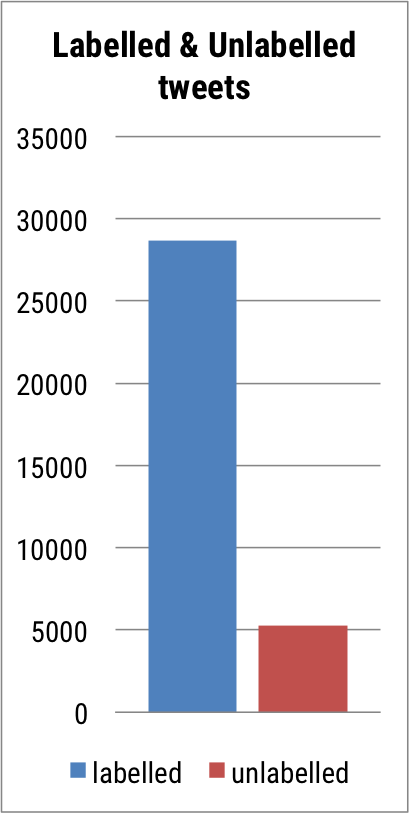
\includegraphics[width=0.25\textwidth]{EmotionLabel}
\caption{The result of Emotion Analysis on the experiment dataset}
\label{fig:emotionLabel}
\end{figure}

Among the labelled tweets, the number of tweets in each emotion was not equally distributed as can be seen in Figure \ref{fig:emotionDistributionWeek}. This finding further supports the argument mentioned in Chapter \ref{ch:approach} that the users tend to post more happy tweets than the other emotions. Within the 10 hour period of the event, the dominating emotion was anger (Figure \ref{fig:emotionDistributionEvent}).

\begin{figure}[htb!] 
\centering 
\begin{subfigure}{0.5\textwidth}
\centering
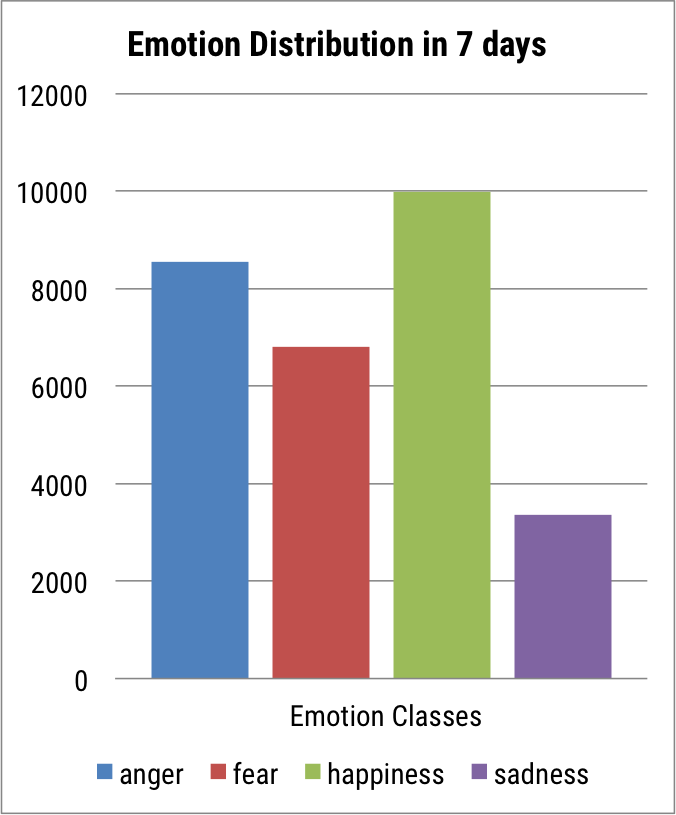
\includegraphics[width=0.8\linewidth]{EmotionDistributionWeek}
\caption{Seven days}
\label{fig:emotionDistributionWeek}
\end{subfigure}%
\begin{subfigure}{0.5\textwidth}
\centering
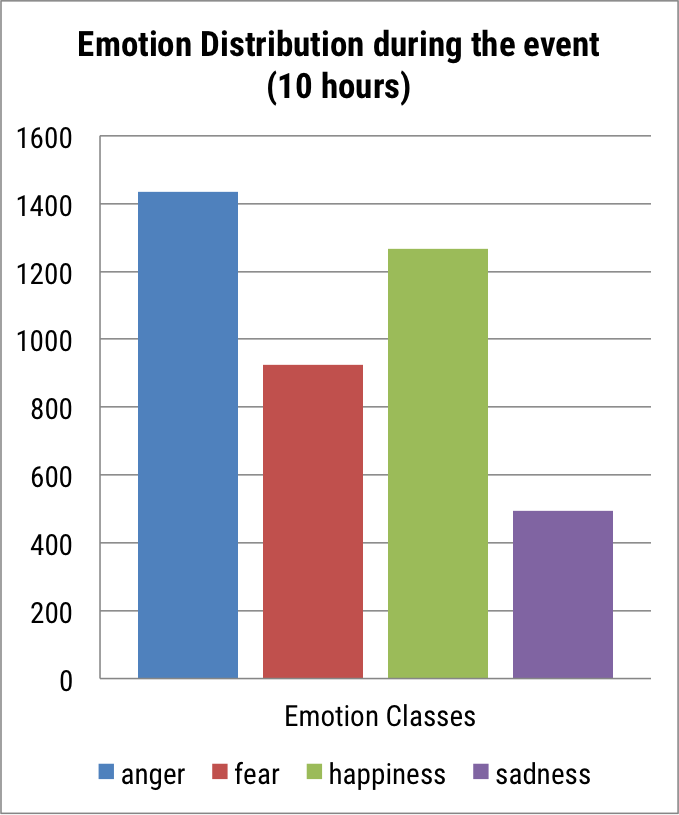
\includegraphics[width=0.8\linewidth]{EmotionDistributionEvent}
\caption{During event}
\label{fig:emotionDistributionEvent}
\end{subfigure}
\caption{The number of tweets labelled with each emotion during the event (b) and in the whole dataset (a)}
\end{figure}

As the objective of the experiment was to evaluate the framework's capability to detect the crowd types during the event, the rest of the analysis mainly focused on the chosen 10 hour period.

\subsection{Emotion Distribution over time}
The tweets were then plotted into each 15 minute interval to observe the change over time.

The number of instance labelled in each emotion over time during the event.
\begin{figure}[htb!] 
\centering
\begin{subfigure}{0.5\textwidth}
\centering
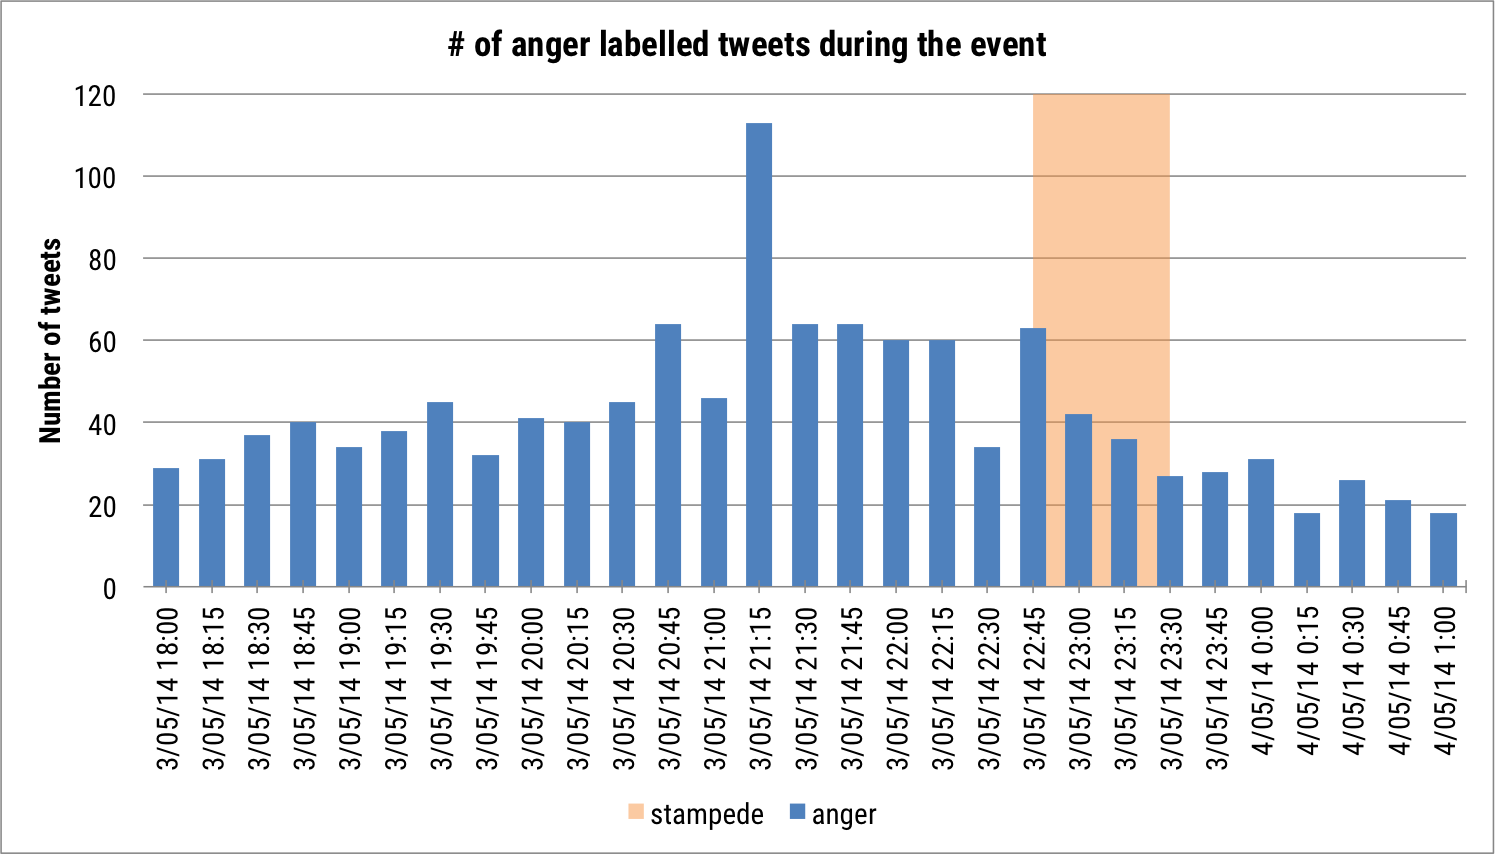
\includegraphics[width=0.98\linewidth]{AngerInstanceEvent}
\caption{anger}
\label{fig:angerInstanceEvent}
\end{subfigure}%
\begin{subfigure}{0.5\textwidth}
\centering    
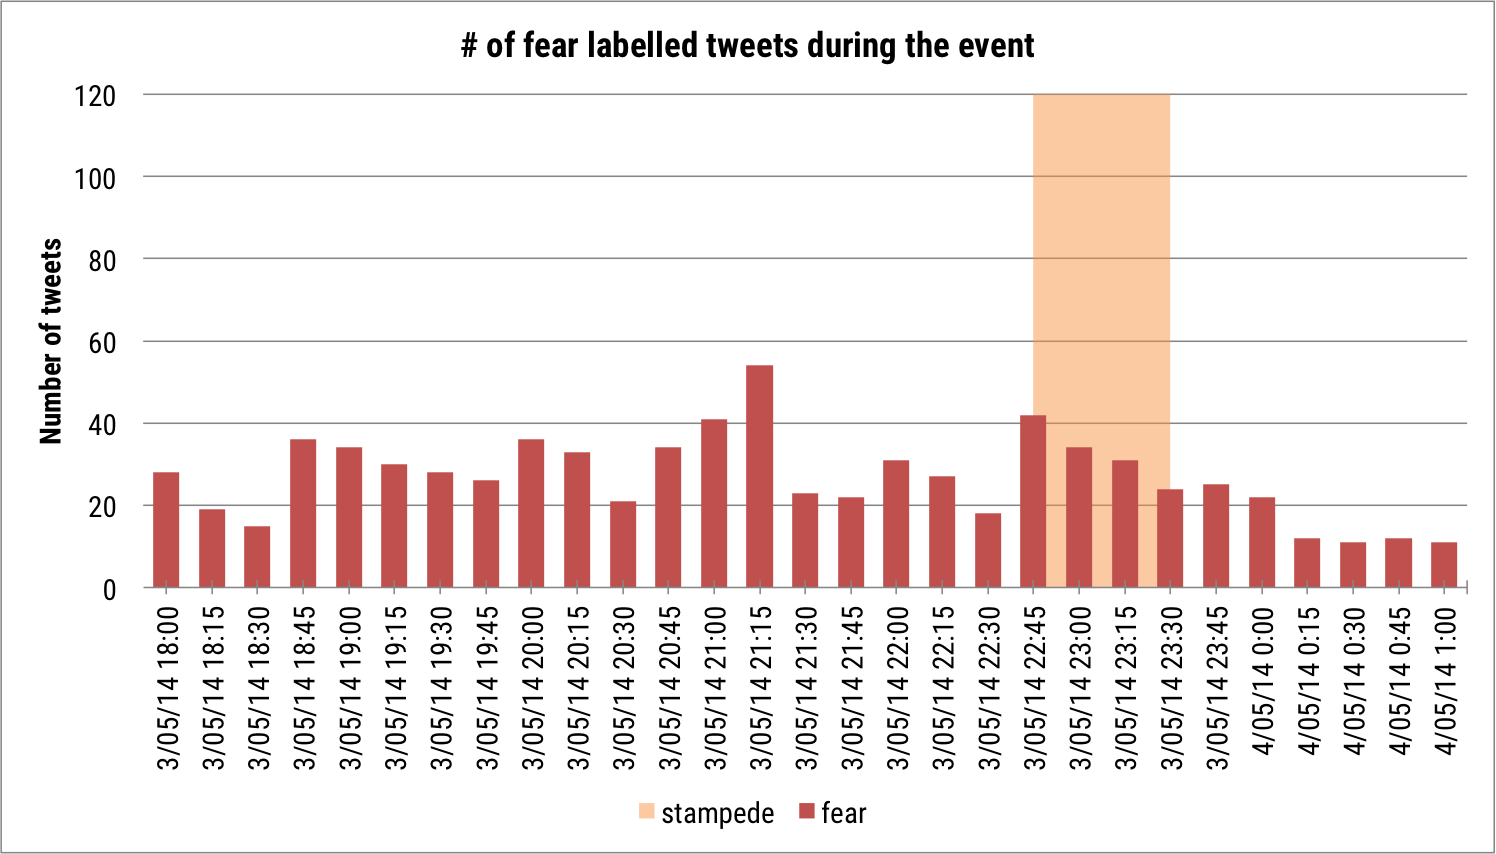
\includegraphics[width=0.98\linewidth]{FearInstanceEvent}
\caption{fear}
\label{fig:fearInstanceEvent}
\end{subfigure}

\begin{subfigure}{0.5\textwidth}
\centering    
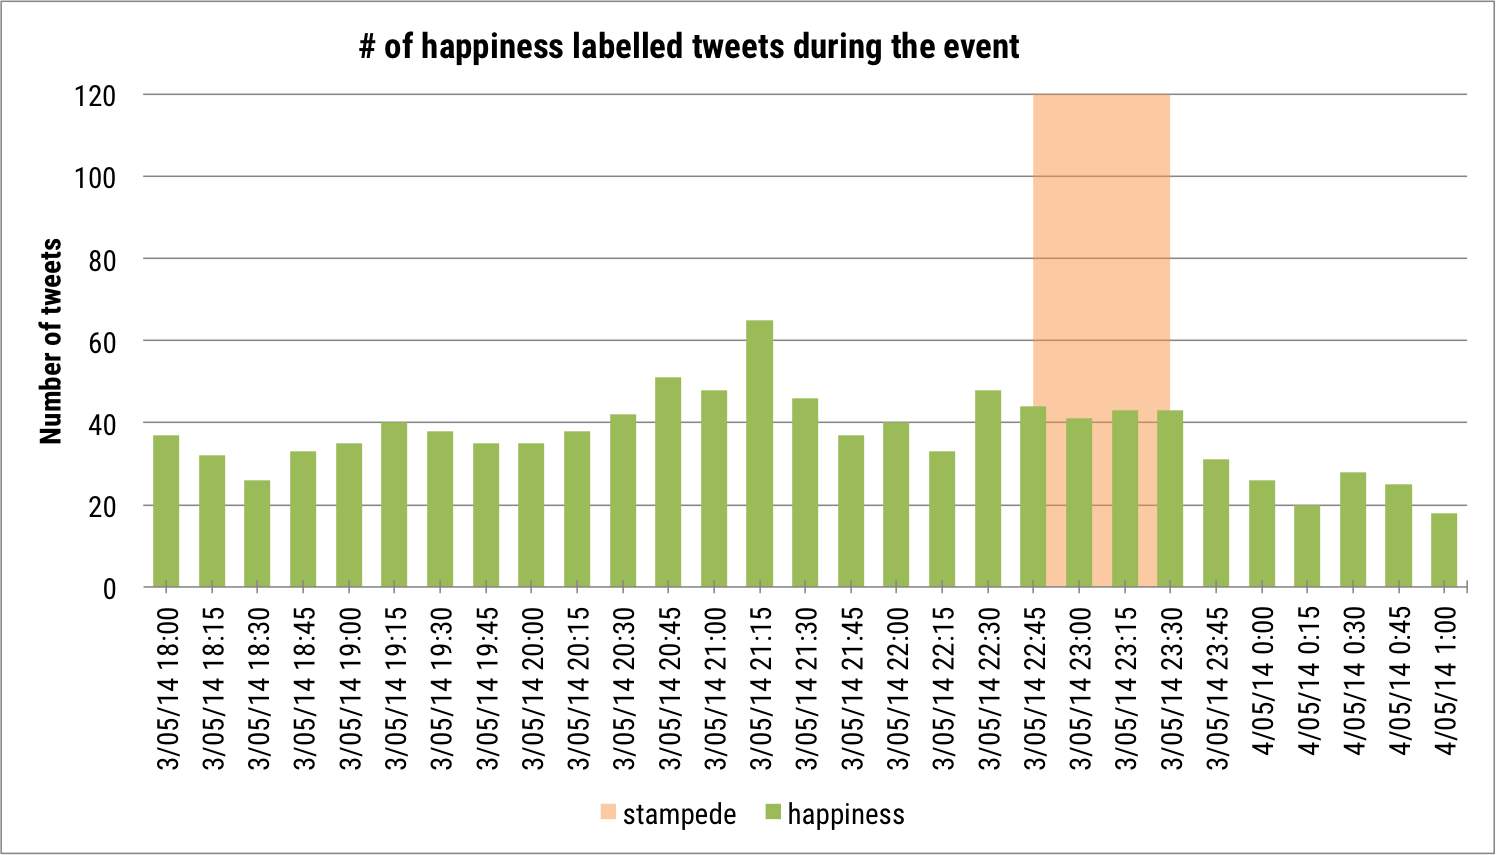
\includegraphics[width=0.98\linewidth]{HappinessInstanceEvent}
\caption{happiness}
\label{fig:happinessInstanceEvent}
\end{subfigure}%
\begin{subfigure}{0.5\textwidth}
\centering    
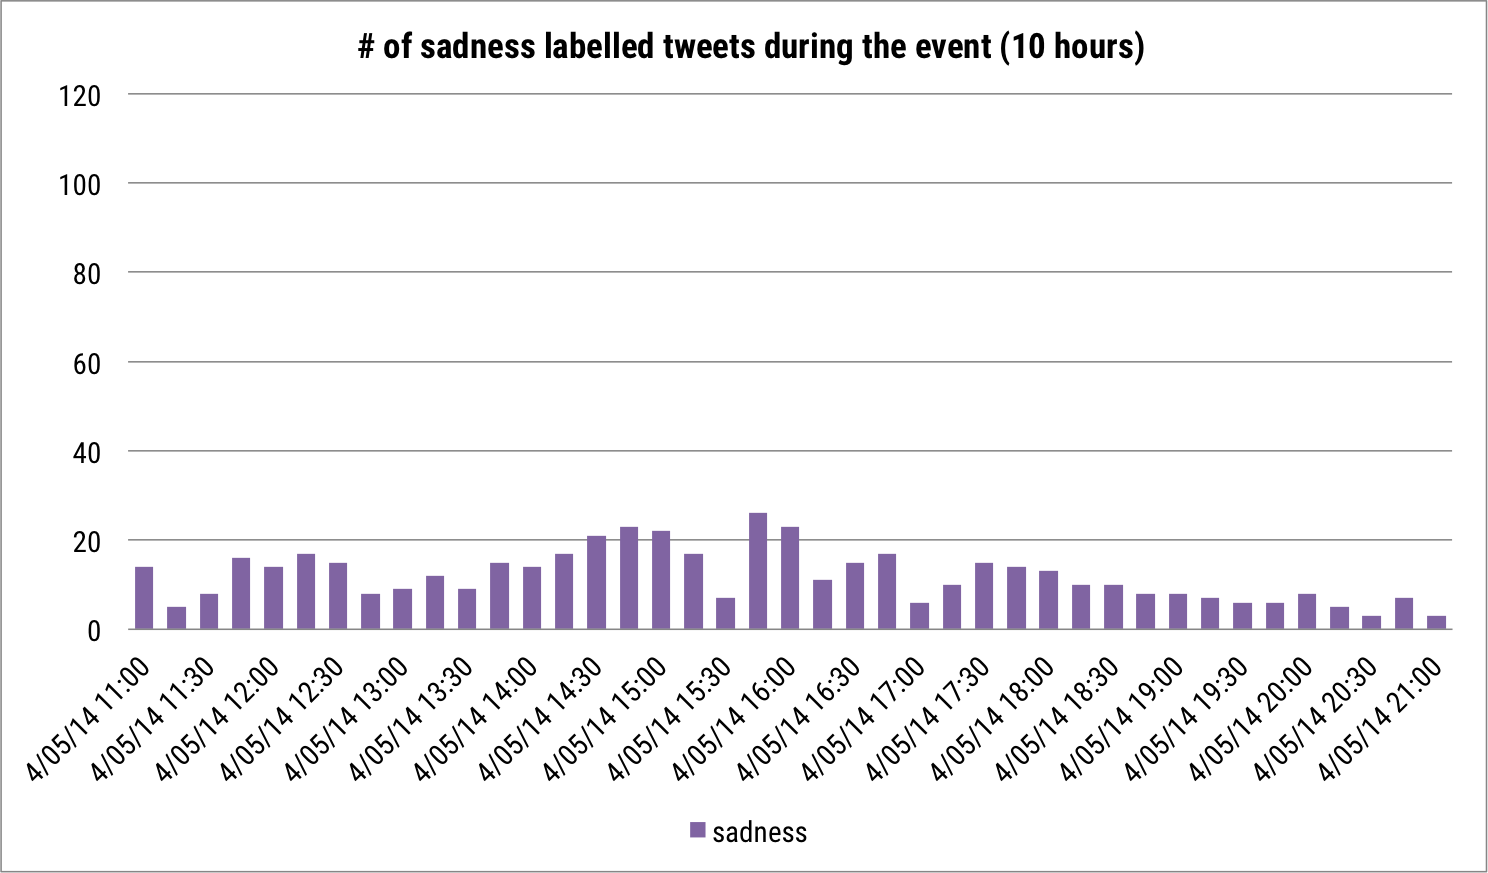
\includegraphics[width=0.98\linewidth]{SadnessInstanceEvent}
\caption{sadness}
\label{fig:sadnessInstanceEvent}
\end{subfigure}
\caption{The number of tweets labelled with anger, fear, happiness and sadness over time during the event}
\end{figure}

The percentage of each emotion over time during the event.
\clearpage
\begin{figure}[htb!] 
\centering    
\begin{subfigure}{0.5\textwidth}
\centering
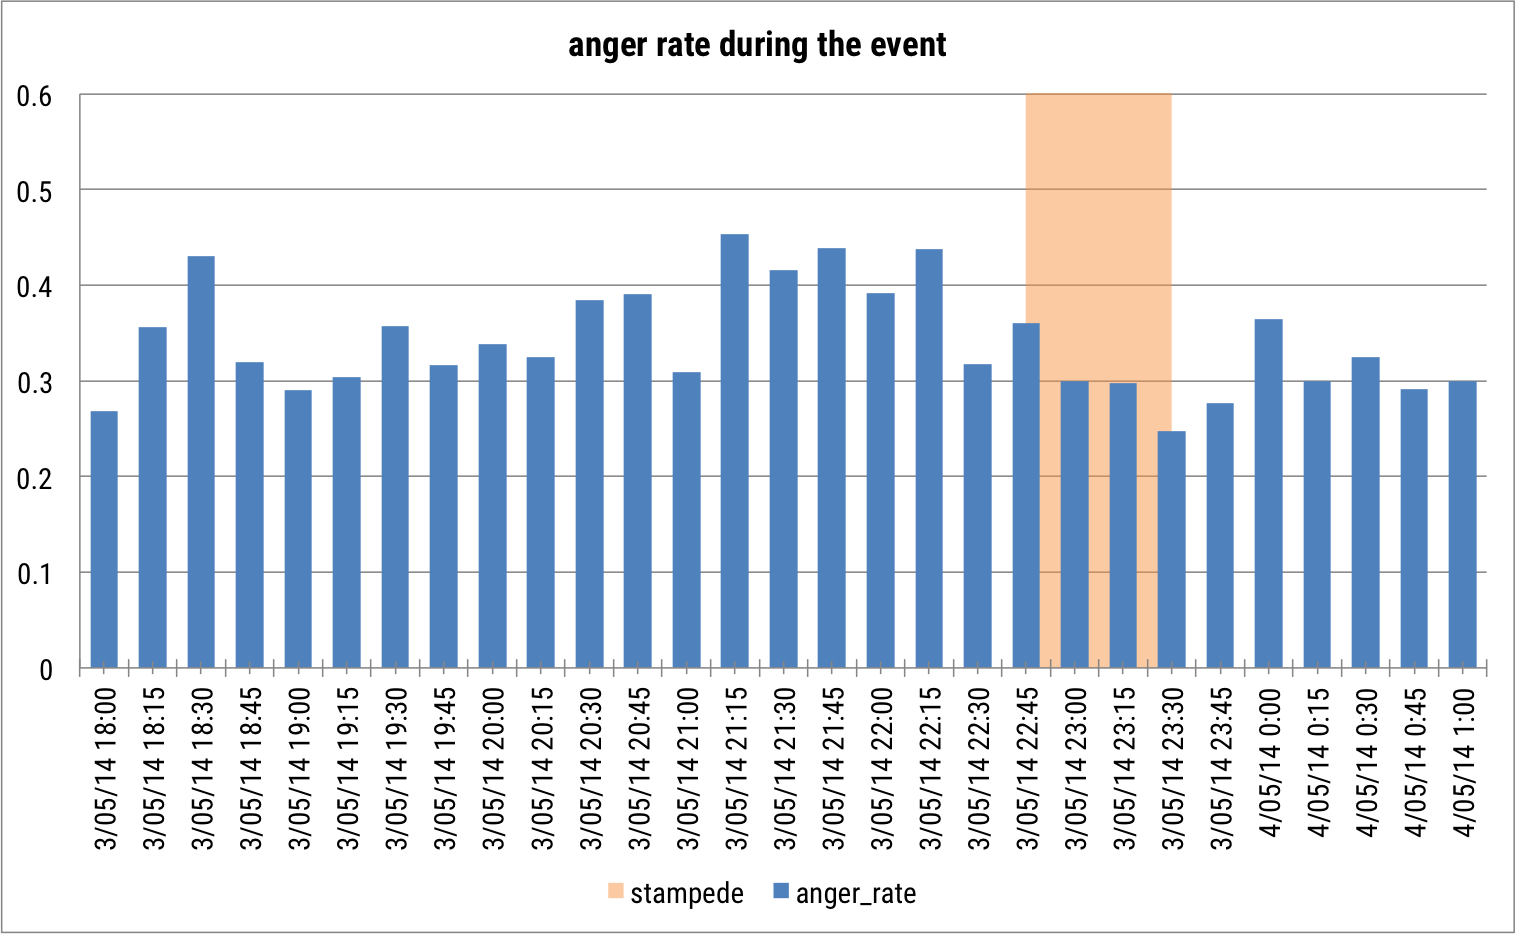
\includegraphics[width=0.98\linewidth]{AngerRateEvent}
\caption{anger}
\label{fig:angerRateEvent}
\end{subfigure}%
\begin{subfigure}{0.5\textwidth}
\centering    
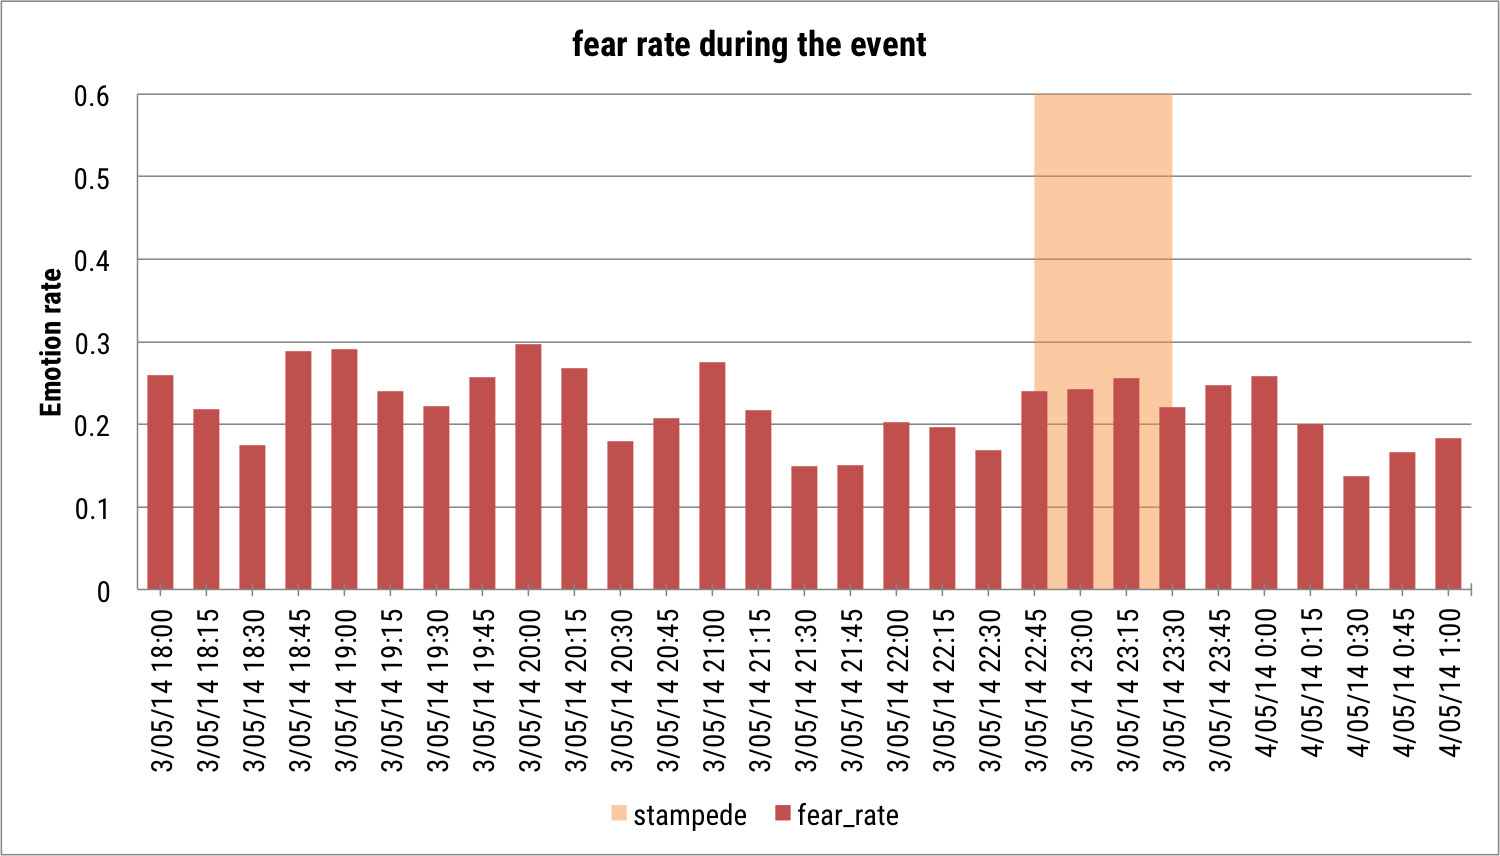
\includegraphics[width=0.98\linewidth]{FearRateEvent}
\caption{fear}
\label{fig:fearRateEvent}
\end{subfigure}

\begin{subfigure}{0.5\textwidth} 
\centering    
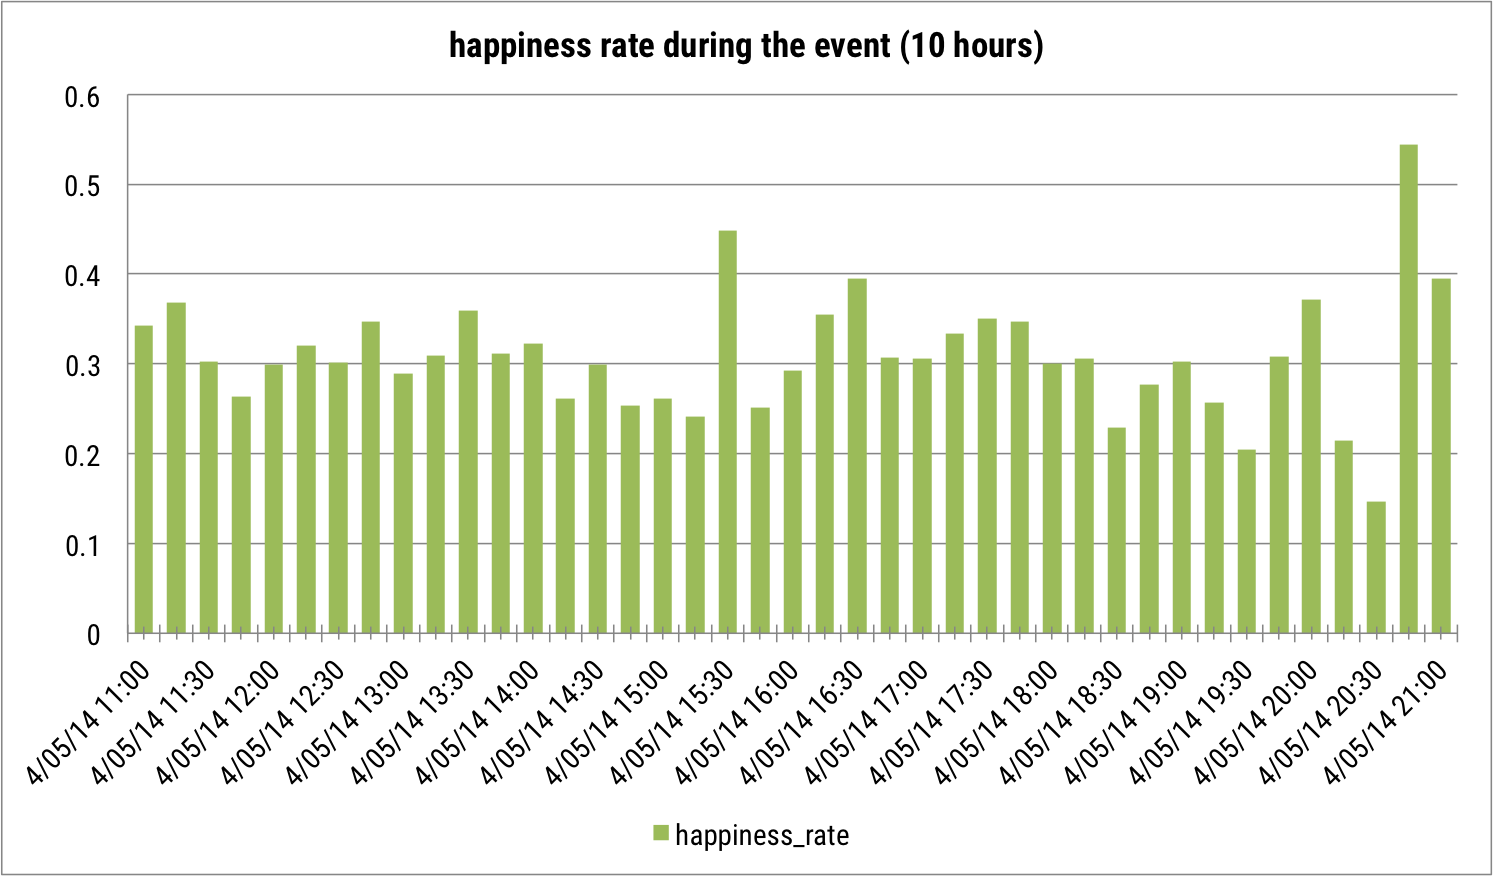
\includegraphics[width=0.98\linewidth]{HappinessRateEvent}
\caption{happiness}
\label{fig:happinessRateEvent}
\end{subfigure}%
\begin{subfigure}{0.5\textwidth}
\centering    
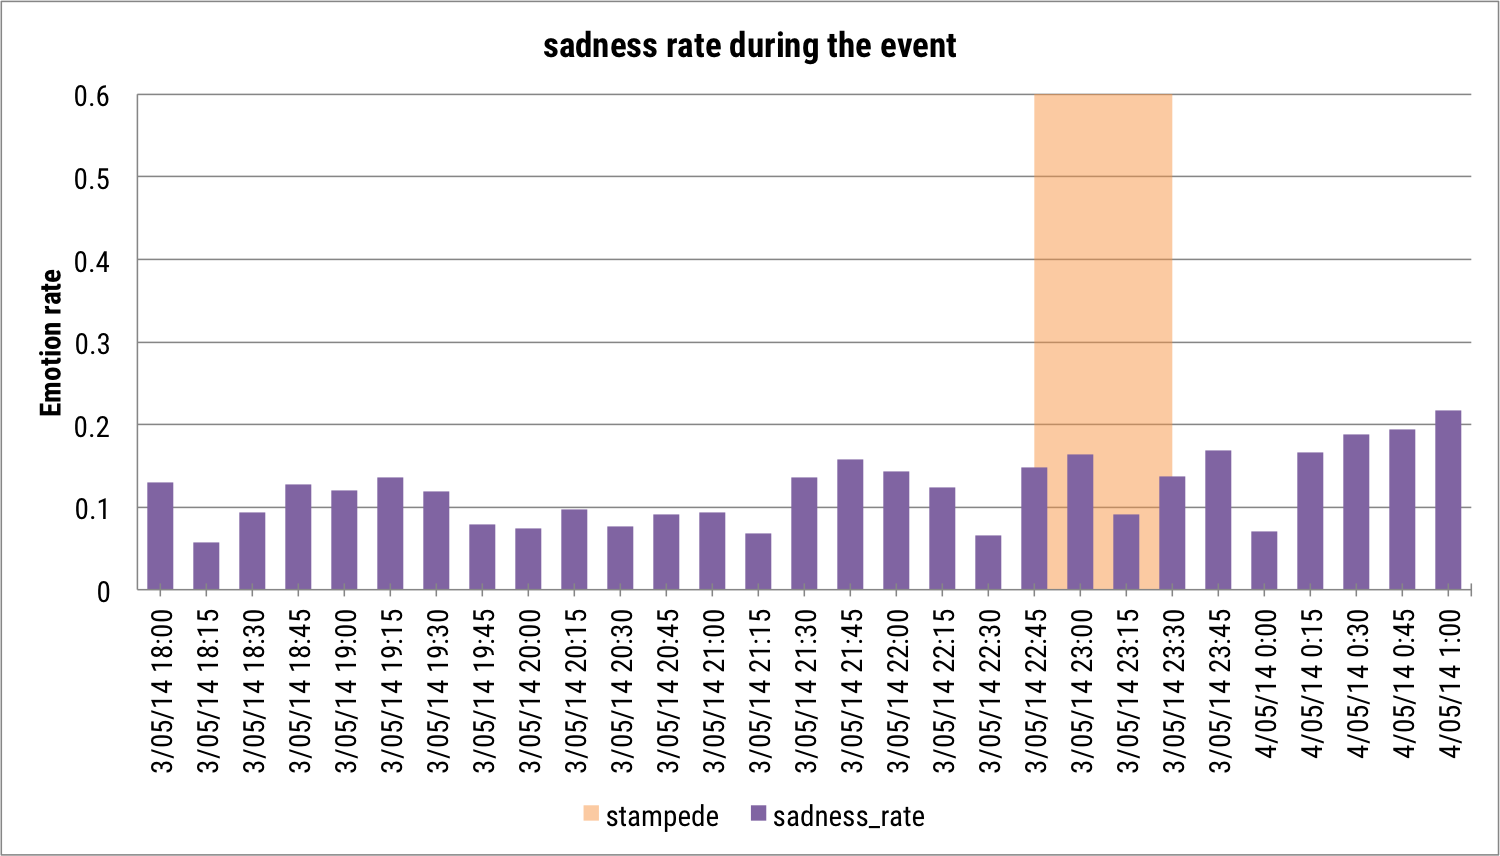
\includegraphics[width=0.98\linewidth]{SadnessRateEvent}
\caption{sadness}
\label{fig:sadnessRateEvent}
\end{subfigure}
\caption{The percentage of anger, fear, happiness and sadness over time during the event}
\end{figure}

\subsubsection{The Normal Distribution of Emotion Rate over time}
Applying histogram to rate over time of each emotion, the normal distribution of the rate can be noticed.

\begin{figure}[htb!] 
\centering    
\begin{subfigure}{0.5\textwidth}
\centering
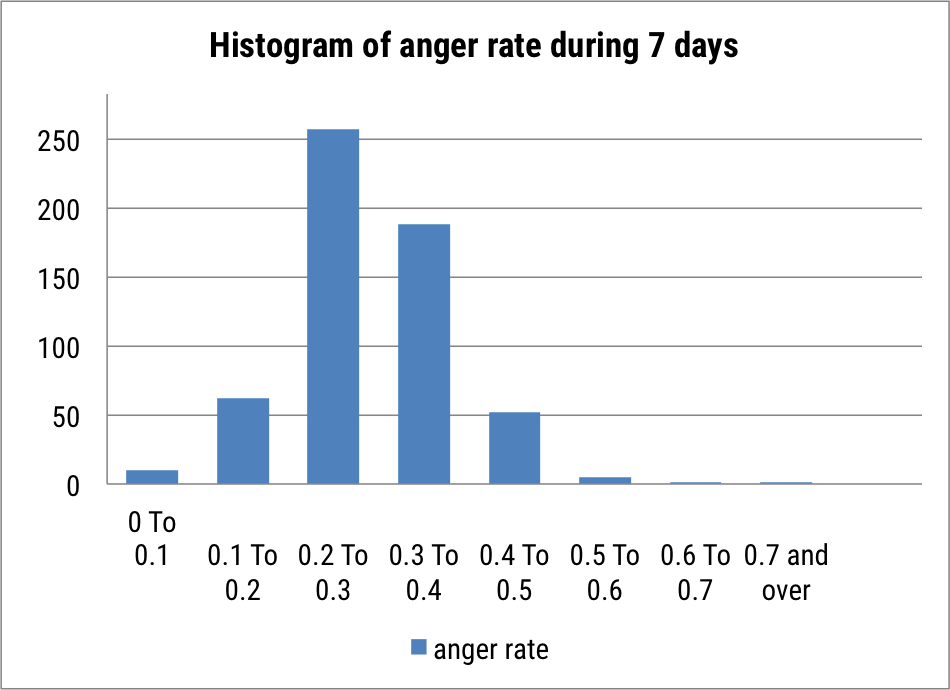
\includegraphics[width=0.8\linewidth]{HistogramAngerWeek}
\caption{anger}
\label{fig:histogramAngerWeek}
\end{subfigure}%
\begin{subfigure}{0.5\textwidth}
\centering    
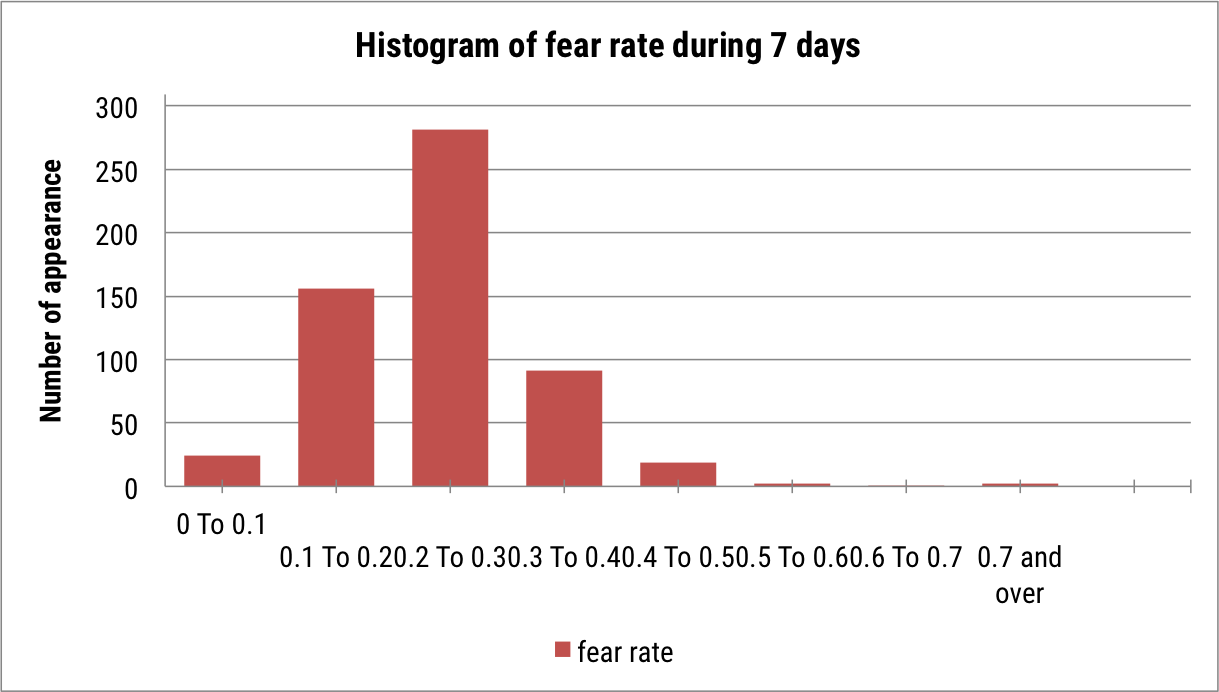
\includegraphics[width=0.8\linewidth]{HistogramFearWeek}
\caption{fear}
\label{fig:histogramFearWeek}

\end{subfigure}
\begin{subfigure}{0.5\textwidth}
\centering    
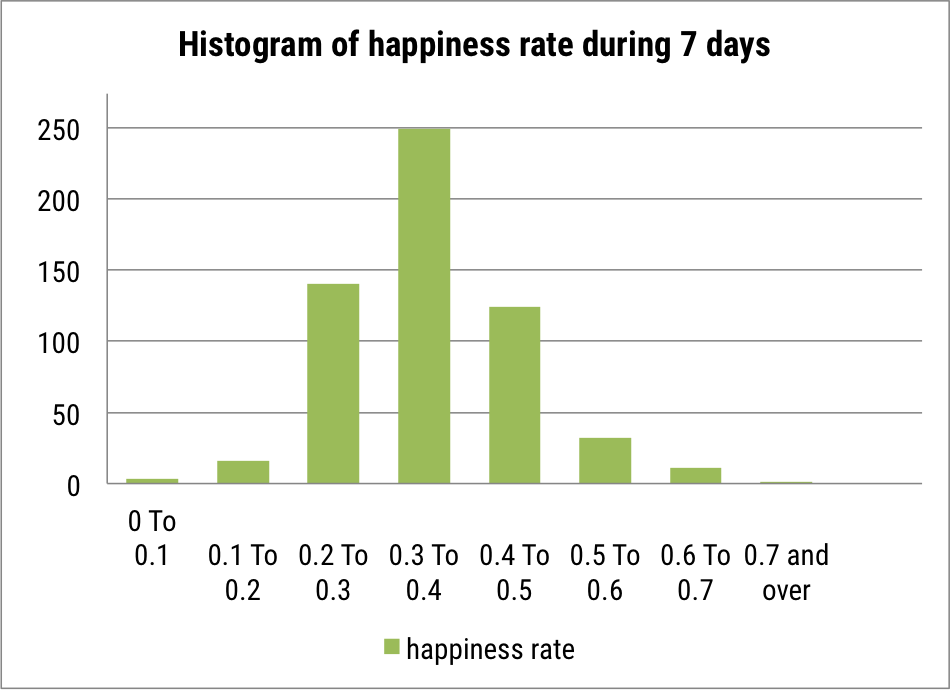
\includegraphics[width=0.8\linewidth]{HistogramHappinessWeek}
\caption{happiness}
\label{fig:histogramHappinessWeek}
\end{subfigure}%
\begin{subfigure}{0.5\textwidth}
\centering    
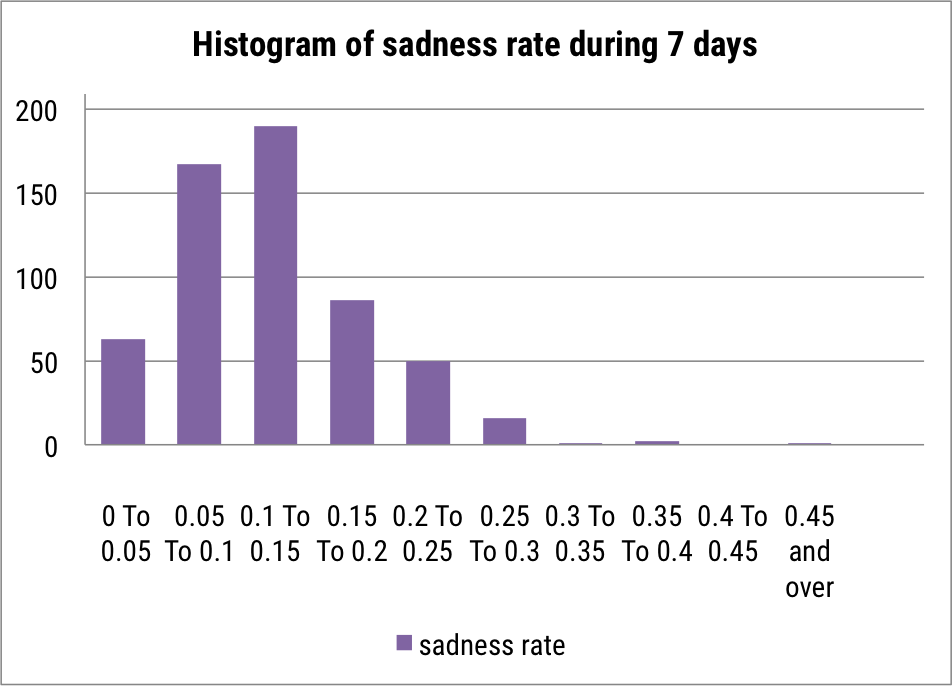
\includegraphics[width=0.8\linewidth]{HistogramSadnessWeek}
\caption{sadness}
\label{fig:histogramSadnessWeek}
\end{subfigure}
\caption{The normal distribution of anger (a), fear (b), happiness (c) and sadness (d) rate over time in the dataset}
\label{fig:histogramWeek}
\end{figure}

\subsubsection{Moving Average, Z-score and the Level of Density of an Emotion}
Set window for moving average as minus 1 hour, which means the mean value is calculate by considering 1 hour of data earlier.
Set the threshold for high level of density of an emotion as z-score = 1, which means this value is higher than the mean value by one standard deviation.
\begin{figure}[htb!] 
\centering   
\begin{subfigure}{0.5\textwidth}
\centering    
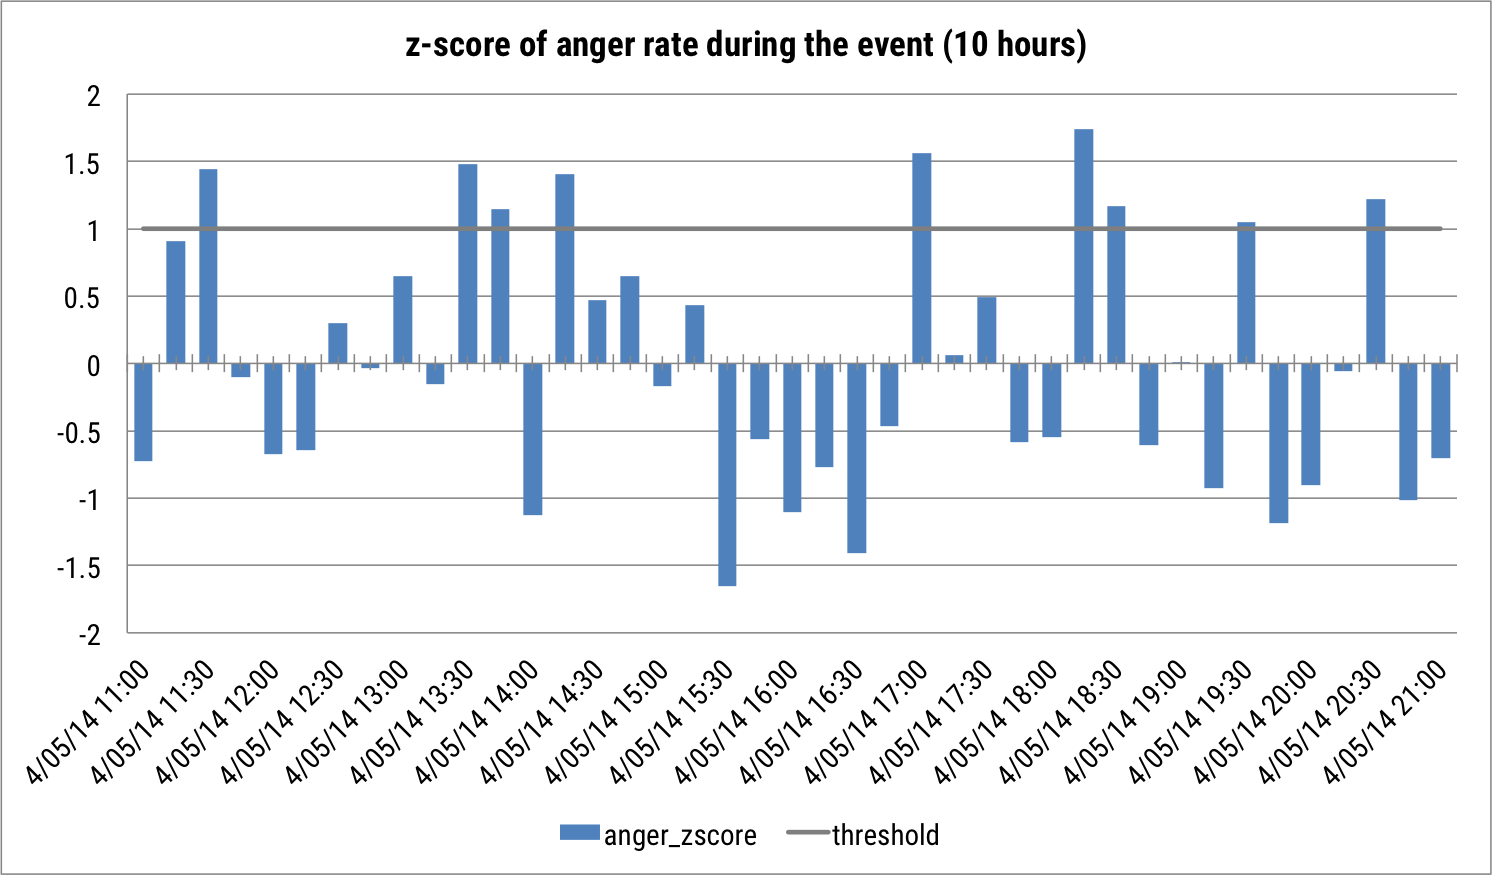
\includegraphics[width=0.98\linewidth]{AngerZscoreEvent}
\caption{anger}
\label{fig:angerZscoreEvent}
\end{subfigure}%
\begin{subfigure}{0.5\textwidth}
\centering    
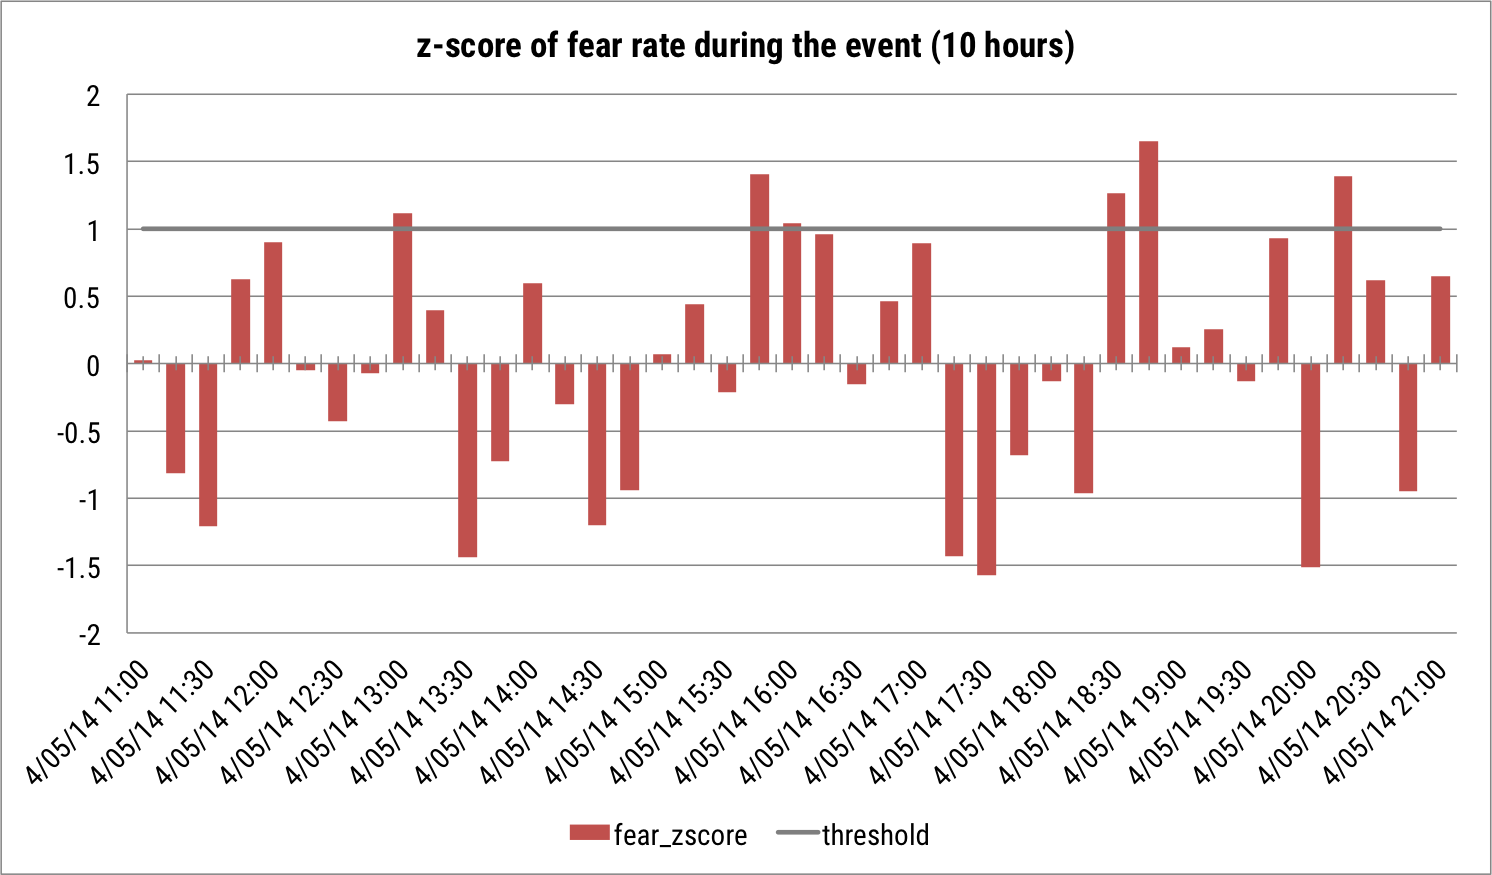
\includegraphics[width=0.98\linewidth]{FearZscoreEvent}
\caption{fear}
\label{fig:fearZscoreEvent}
\end{subfigure}

\begin{subfigure}{0.5\textwidth}
\centering    
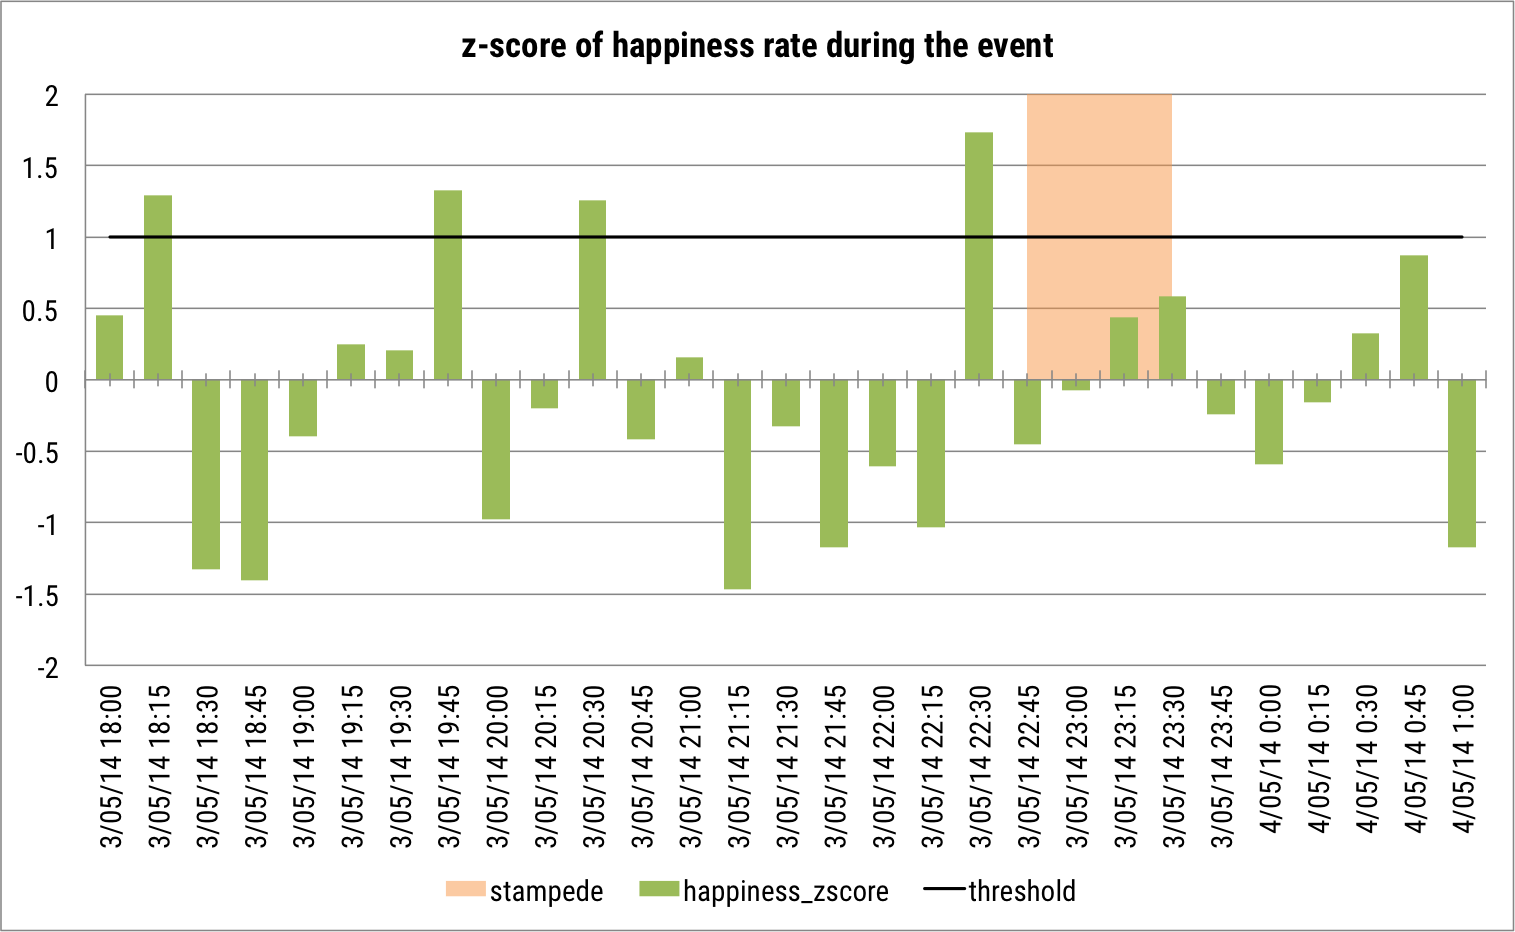
\includegraphics[width=0.98\linewidth]{HappinessZscoreEvent}
\caption{happiness}
\label{fig:happinessZscoreEvent}
\end{subfigure}%
\begin{subfigure}{0.5\textwidth}
\centering    
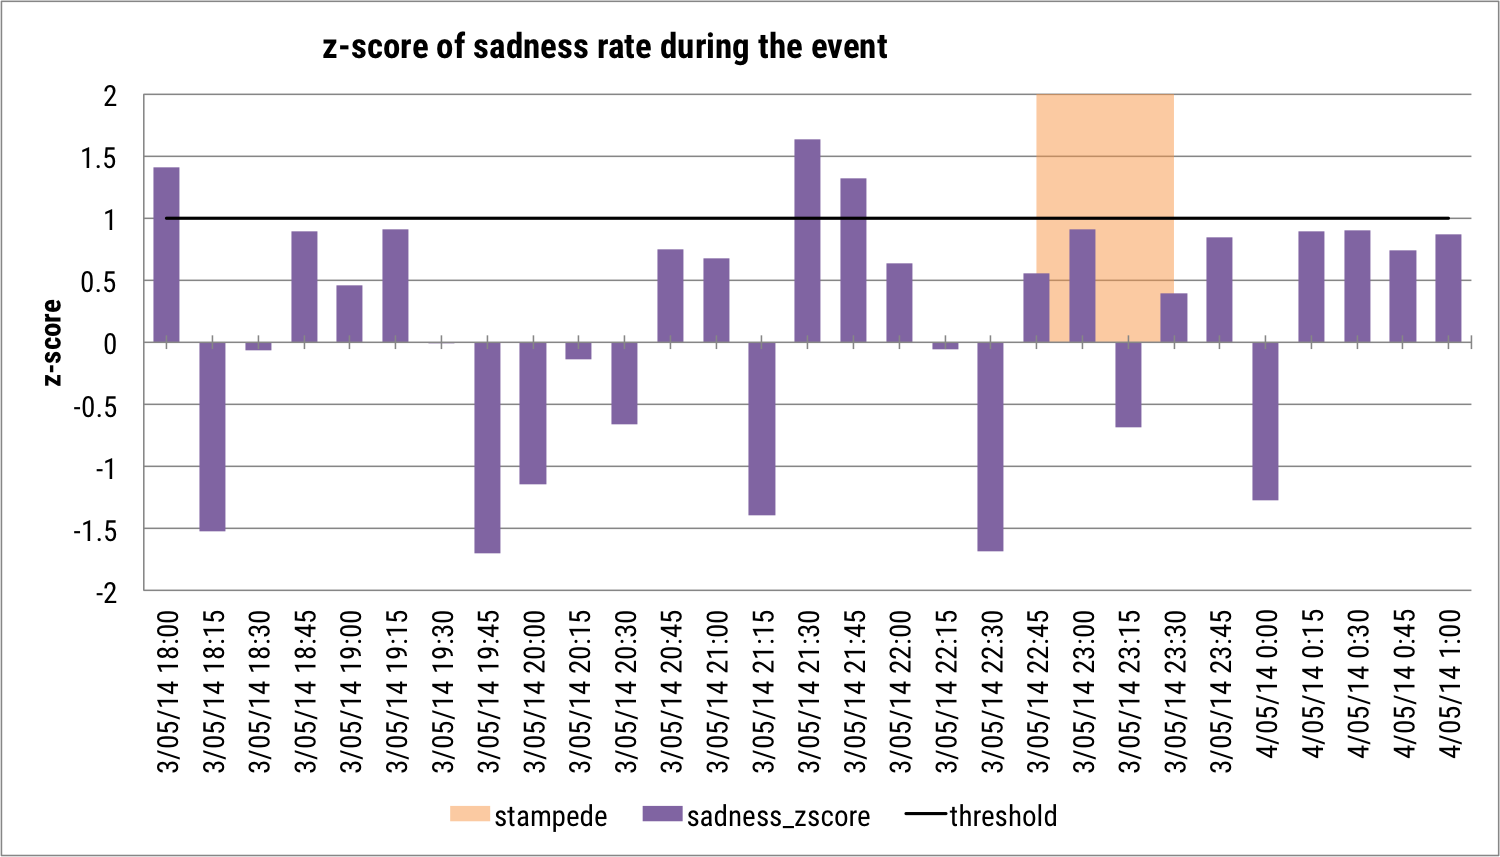
\includegraphics[width=0.98\linewidth]{SadnessZscoreEvent}
\caption{sadness}
\label{fig:sadnessZscoreEvent}
\end{subfigure}
\caption{The z-score of anger, fear, happiness and sadness rate over time during the event}
\end{figure}

\subsection{Rule Based Reasoning and Possible Crowd Types}

\section{Discussion}

\section{Conclusion}